%\section{Results} 

The measured differential cross-section $d\sigma/dQ^2_{QE}$ is shown in 
Fig.~\ref{fig:xsec_q2} and Table~\ref{tab:xsec}. 
Averaged over the flux from 1.5 to 10~GeV, we find  $\sigma=0.604 \pm 0.008 \mbox{(stat)} \pm 0.075 \mbox{(syst)} \times \unit[10^{-38}]{cm^2/proton}$.  
As noted above, the systematic uncertainties
are significantly reduced in the shape of the differential
cross-section\footnoterecall{footsupp}, which is shown in Fig.~\ref{fig:xsec_q2_shape_ratio}.
%Figures~\ref{fig:xsec_q2} and \ref{fig:xsec_q2_shape_ratio} 

Table~\ref{tab:chi2} compares the data to the RFG model in the 
GENIE event generator and a number of different nuclear models 
and values of $M_A$ in the NuWro generator~\cite{Golan:2012wx}.
%Models incorporating a low $Q^2_{QE}$ suppression 
%in the random phase approximation (RPA)~\cite{Singh1992587,Graczyk:2003ru} 
%underpredict the cross-section at low $Q^2_{QE}$, and 
There
is little sensitivity to replacement of the Fermi gas with
a spectral function (SF) model of the target nucleon energy-momentum
relationship~\cite{Benhar:1994hw}. The data disfavor $M_A=\unit[1.35]{GeV/c^2}$  as extracted from fits of the MiniBooNE neutrino quasi-elastic data
in the RFG model~\cite{AguilarArevalo:2007ab}. Our data are consistent with a transverse enhancement model (TEM) which has $M_A=\unit[0.99]{GeV/c^2}$ in agreement with deuterium data and includes an enhancement of the magnetic form factors of bound nucleons that has been observed in electron-carbon scattering~\cite{Bodek:2011ps}. The $M_A=\unit[1.35]{GeV/c^2}$ and TEM models have a similar $Q^{2}_{QE}$ dependence at low $Q^{2}_{QE}$ but are distinguished by the kinematic reach of the data at $Q^{2}_{QE}>\unit[1]{GeV^2}$.

\begin{figure}[tp]
\centering
\ifnum\PRLsupp=0
  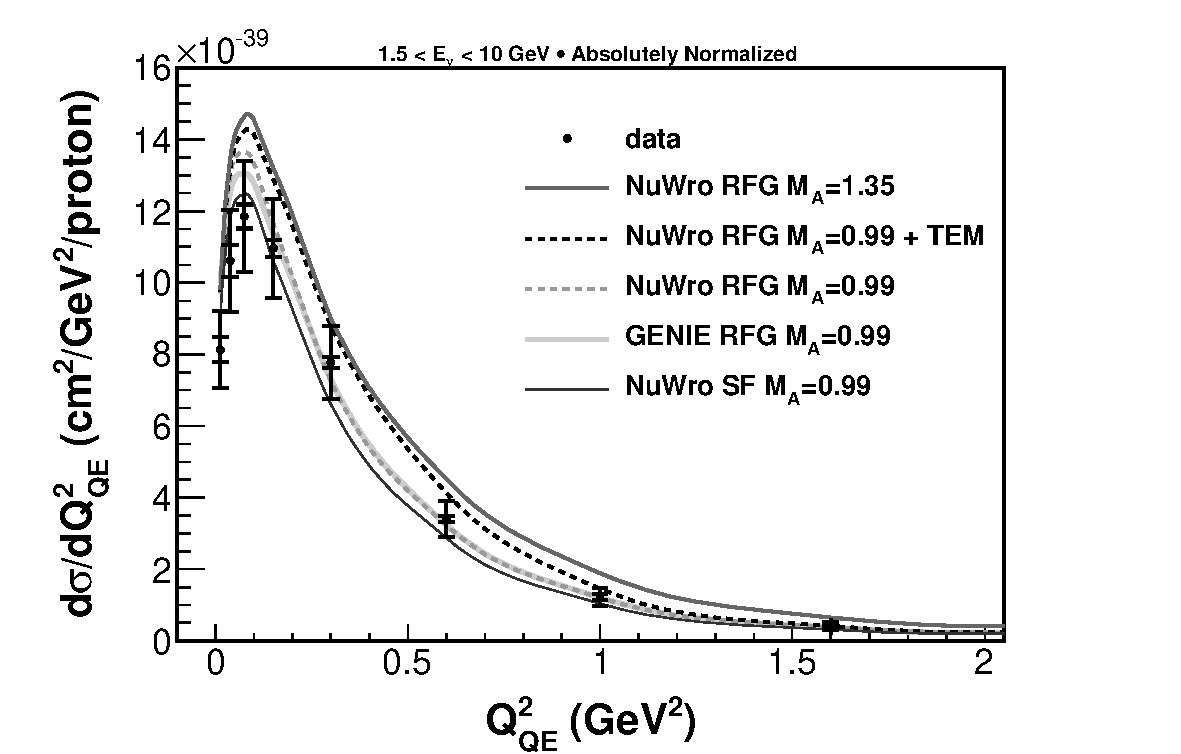
\includegraphics[width=\columnwidth]{figures/Figure3_anu_norpa} 
\else
  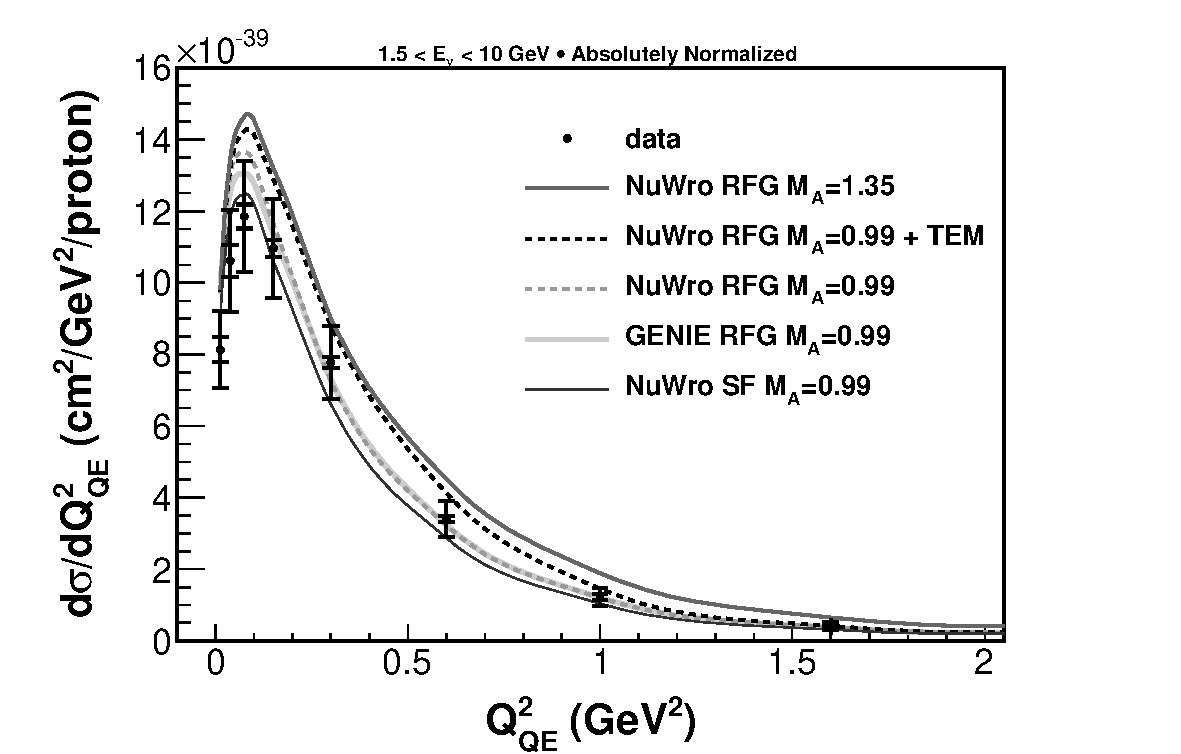
\includegraphics[width=0.8\columnwidth]{figures/Figure3_anu_norpa} 
\fi
%    \vspace{-7pt}
\caption{The anti-neutrino
  quasi-elastic cross-section as a function of $Q^2_{QE}$ compared
  with several different models of the interaction described in the
  text. The inner (outer) error bars correspond to the
  statistical (total) uncertainties.}
%    \vspace{-10pt}
\label{fig:xsec_q2}
\end{figure}
\begin{figure}[tp]
\centering
\ifnum\PRLsupp=0
  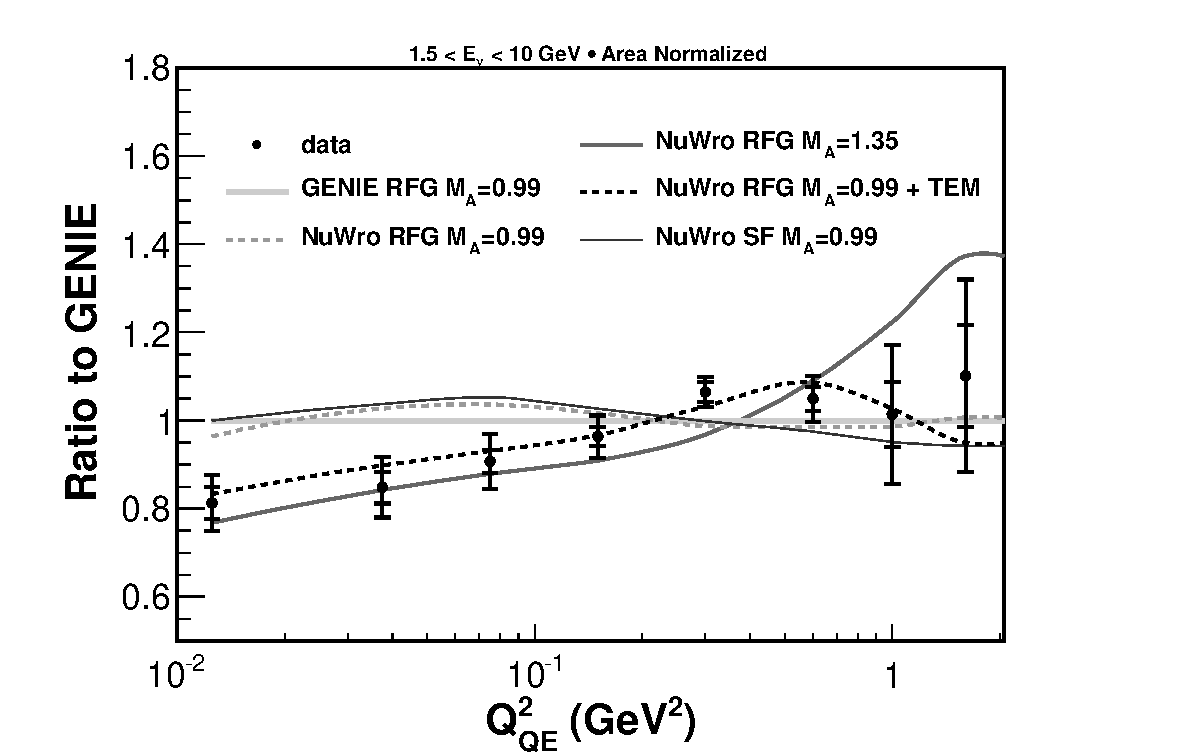
\includegraphics[width=\columnwidth]{figures/Figure4_anu_norpa} 
\else
  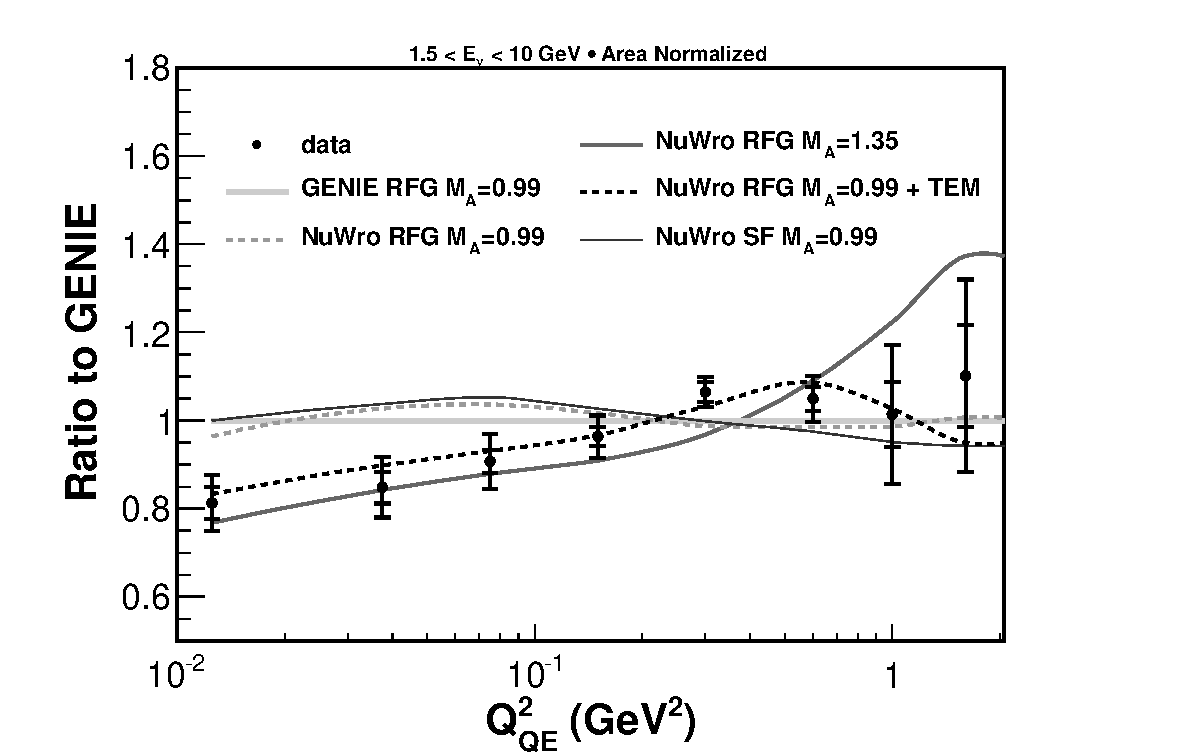
\includegraphics[width=0.8\columnwidth]{figures/Figure4_anu_norpa} 
\fi
\caption{The data and models of Fig.~\ref{fig:xsec_q2} shown by $Q^2_{QE}$ shape and as a ratio to the reference GENIE prediction.}
\label{fig:xsec_q2_shape_ratio}
\end{figure}

\begingroup
\squeezetable
\begin{table}
\begin{tabular}{ccc}
$Q^2_{QE}$ & Cross-section  &  Fraction of \\
{\footnotesize (GeV$^2$) }    & {\footnotesize ($10^{-38}\mathrm{cm}^2/\mathrm{GeV}^2/$proton) } &  Cross-section {\footnotesize (\%)} \\ \hline
$0.0 - 0.025$ & $0.813\pm0.035\pm0.102$ &  $3.45\pm0.15\pm0.22$ \\ 
$0.025 - 0.05$ & $1.061\pm0.045\pm0.134$ &  $4.50\pm0.19\pm0.31$ \\ 
$0.05 - 0.1$ & $1.185\pm0.033\pm0.150$ &  $10.05\pm0.28\pm0.63$ \\ 
$0.1 - 0.2$ & $1.096\pm0.024\pm0.135$ &  $18.59\pm0.41\pm0.83$ \\ 
$0.2 - 0.4$ & $0.777\pm0.016\pm0.101$ &  $26.38\pm0.55\pm0.62$ \\ 
$0.4 - 0.8$ & $0.340\pm0.009\pm0.050$ &  $23.11\pm0.61\pm0.98$ \\ 
$0.8 - 1.2$ & $0.123\pm0.009\pm0.024$ &  $8.35\pm0.61\pm1.15$ \\ 
$1.2 - 2.0$ & $0.041\pm0.004\pm0.010$ &  $5.57\pm0.59\pm0.94$ \\ 
\hline
\end{tabular}
\caption{Table of absolute and shape-only cross-section results.  In each measurement, the first error is statistical and the second is systematic.}
\label{tab:xsec}
\end{table}
\endgroup


\begingroup 
\squeezetable 
\begin{table} 
\begin{tabular}{c|cccc}
NuWro  &  ~RFG~ & ~RFG~  & ~RFG~ & ~SF~ \\  
Model   &          & +TEM~  & &  \\ \hline
$M_A$ (GeV) &  0.99 & 0.99 & 1.35 & 0.99  \\  \hline \hline
%Rate $\chi^2$  & 21.1 & 8.46 & 23.2 & 17.1  \\ 
%Shape $\chi^2$ & 20.3 & 4.59 & 12.1 & 20.9 \\
Rate $\chi^2$/d.o.f. & 2.64 & 1.06 & 2.90 & 2.14 \\
Shape $\chi^2$/d.o.f. & 2.90 & 0.66 & 1.73 & 2.99  \\
%FGM & 0.99 & 33.8 & 30.2 & 33.4 & 36.5 \\ 
%FGM + TEM & 0.99 & 10.3 & 21.7 & 6.29 & 18.1 \\ 
%FGM & 1.35 & 29.3 & 30.7 & 16.9 & 23.6 \\ 
%SF & 0.99 & 28.8 & 24.2 & 34.3 & 34.2 \\ 
%RPA & 0.99 & 24.5 & 75.8 & 27.2 & 91.9 \\ 
\end{tabular}
\caption{\label{tab:chi2} Comparisons between the measured $d\sigma/dQ^2_{QE}$ (or its shape in $Q^2_{QE}$) and different models implemented using the NuWro neutrino event generator, expressed as $\chi^2$ per degree of freedom (d.o.f.) for eight (seven) degrees of freedom.  The $\chi^2$ computation in the table accounts for significant 
correlations between the data points caused by systematic uncertainties. }
%\caption{\label{tab:chi2} $\chi^2$ statistic for eight (seven) degrees of %freedom for comparison between the measured $d\sigma/dQ^2_{QE}$, as well as its %shape in $Q^2_{QE}$, and different models implemented using the NuWro neutrino %event generator. The $\chi^2$ computation accounts for significant 
%correlations between the data points caused by systematic uncertainties.
%}%, for both neutrino and antineutrino modes.
\end{table}
\endgroup

